\section{Voice communication system} \label{sec:link_budget}
In order to establish voice communication -- and at a later stage data communication\footnote{Data communication is not covered in this thesis.} -- it was decided to use the VHF band.\footnote{The VHF band has a frequency range from $30\mathrm{MHz}$ to $300\mathrm{MHz}$.} It is preferred for mobile and handheld radio applications, as the range is relatively short and only extends over a few tens of kilometers. With regard to this, the possible interference with neighboring communication systems can be kept to a minimum \cite{Parsons:2000}. Since the OeWF already uses handheld radios that operate in the VHF band, it was decided to incorporate them into the voice communication system due to their good condition.

In the past, VHF radios mainly used analog modulation methods for signal transmission. Nowadays, however, it is an increasing trend in this industry to use digital modulation methods. These have the decisive advantage that the signal quality -- for example the audio quality -- remains relatively constant up to a certain distance and then deteriorated drastically. In the case of radios that transmit an analog modulated signal, the quality of the signal constantly deteriorates with increasing distance \cite{SystemPlanner:2018}. So that good audio quality over longer distances can be guaranteed the decision was made to use a radio infrastructure based on digital modulation. 

In combination with the aforementioned infrastructure, vertically polarized omnidirectional antennas were preferred because the field strength near the ground is stronger than that of horizontally polarized antennas. Moreover, these antennas are often more convenient to use and their directivity is the same for all cardinal directions -- in relation to the insatallation site of a radio system or the current location of a handheld radio \cite{Parsons:2000}. 

Communication with frequencies in the VHF range has the consequence that the radio waves only propagate -- from the transmitter to the receiver -- via a direct \emph{line of sight} (LOS) and above the ground as ground waves. As will be shown later, the latter contribute more to the link budget. Ionospheric propagation does not occur in this band because the frequencies are too high \cite{Parsons:2000}. 

The following subsections deal with the important equations and relationships required to model a voice communication system based on the facts just mentioned. 

% ADD HERE

\subsection{Load for the electrical energy distribution} \label{sec:load_radio}
In the section \ref{sec:methodology} the self-sufficient energy distribution system for the voice communication system was presented. The electrical load of the energy distribution system is a radio device -- for example a repeater or a mobile radio -- that operates independently of other energy sources with a certain duty cycle $a_\mathrm{T}/a_\mathrm{R}/a_\mathrm{Stby}$ in $\left(\%\right)$. The duty cycle gives an indication of what percentage of the operating time the device is in transmission, receiving or standby mode. Since its current consumption is usually specified in the data sheet together with the associated operating mode, the load current $I_\mathrm{L}$ can be generalized as follows \cite{DM2600:2013, SLR1000:2019}: 
\begin{equation} \label{eq:battery_current}
	\centering
	I_\mathrm{L}(t) =
  	\begin{cases}
   		I_\mathrm{T}(t)\text{,} & \text{when the load transmits} \\
    	I_\mathrm{R}(t)\text{,} & \text{when the load receives} \\
		I_\mathrm{Stby}(t)\text{,} & \text{when the load is in standby}
 	\end{cases}
\end{equation}  

For a desired duty cycle, the current consumption of the device can then be modeled with a simple step function. It is assumed that the device installed on site -- which is supplied by the self-sufficient energy distribution system -- is not shut down outside of operating hours. During these hours it consumes $I_\mathrm{Stby}$. 
\subsection{Free space signal budget}
This subsection repeats the basics of the free space signal budget. It is assumed that there are no obstacles in the beam path between a transmitter and a receiver radio, and that their antennas are separated by the \emph{distance} $d$ in $\left(\mathrm{m}\right)$. The \emph{available power} $P_\mathrm{R}$ in $\left(\mathrm{W}\right)$ at the receiving antenna with the \emph{gain} $G_\mathrm{R}$ in $\left(\mathrm{1}\right)$ and the \emph{receiving losses} $L_\mathrm{R}$ in $\left(\mathrm{1}\right)$ -- which are caused by, for example, coaxial cables, connectors, adapters or lightning arresters in the antenna feed line -- can then be calculated based on the \emph{transmission power} $P_\mathrm{T}$ in $\left(\mathrm{W}\right)$, the gain of the transmission antenna $G_\mathrm{T}$ in $\left(\mathrm{1}\right)$, the \emph{transmission losses} $L_\mathrm{T}$ in $\left(\mathrm{1}\right)$ -- which are of the same nature as the receiving losses -- and the \emph{free space basic transmission loss} between isotropic antennas $L_\mathrm{ISO}$ in $\left(\mathrm{1}\right)$, while considering the \emph{wavelength} $\lambda_\sim$ in $\left(\mathrm{m}\right)$ of the transmitted electromagnetic wave, as shown in the equation (\ref{eq:free_space}).
\begin{equation} \label{eq:free_space}
	\centering
	P_\mathrm{R} = P_\mathrm{T} \underbrace{\left(\dfrac{\lambda_\sim}{4 \pi \, d}\right)^2}_{L_\mathrm{ISO}^{-1}} L_\mathrm{R} \, L_\mathrm{T} \, G_\mathrm{R} \, G_\mathrm{T}
\end{equation}
When the equation (\ref{eq:free_space}) is expressed in decibels, it can be converted into a simple summation:
\begin{equation} \label{eq:free_space_dB}
	\centering
	P_\mathrm{R,dBW} = P_\mathrm{T,dBW} + \underbrace{20\mathrm{dB} \cdot \log_{10} \left(\dfrac{\lambda_\sim}{4 \pi \, d}\right)}_{- L_\mathrm{ISO,dB}} - L_\mathrm{R,dB} - L_\mathrm{T,dB} + G_\mathrm{R,dBi} + G_\mathrm{T,dBi}\text{.}
\end{equation}
The transmission and available power $P_\mathrm{T}$ and $P_\mathrm{R}$ use $P_0 = 1\mathrm{W}$ as the reference power. A given power $P$ in $\left(\mathrm{W}\right)$ can therefore be converted into decibels with:
\begin{equation} \label{eq:p_dBW_calc}
	\centering
	P_\mathrm{dBW} = 10\mathrm{dBW} \cdot \log_{10} \left(\dfrac{P}{P_0}\right)\text{.}
\end{equation}
$G_\mathrm{T,dBi}$ and $G_\mathrm{R,dBi}$ in $\left(\mathrm{dBi}\right)$ are the antenna gains with respect to the isotropic radiator. The losses in the antenna feed lines are divided into two groups. First, the insertion losses caused by the signal attenuation due to the individual components in the antenna feed lines, and second, the losses caused by a slight mismatch of the impedances of these components. The latter causes reflections which result in a relative loss of $P_\mathrm{T}$ or $P_\mathrm{R}$. Based on the \emph{voltage standing wave ratio} (VSWR) in $\left(\mathrm{1}\right)$ of a component in the antenna feed line, the component's mismatch loss can be calculated as follows:
\begin{equation} \label{eq:mismatch}
	\centering
	L_\mathrm{M,dB} = - 10\mathrm{dB} \cdot \log_{10} \left( 1 - \left( \dfrac{\mathrm{VSWR} - 1}{\mathrm{VSWR} + 1} \right)^2 \right)\text{.}
\end{equation}
With the number of occurring insertion and mismatch losses in the feed lines of the transmission and receiving antenna $N_\mathrm{I}$ and $N_\mathrm{M}$ in $\left(1\right)$, $L_\mathrm{R,dB}$ and $L_\mathrm{T,dB}$ can now be calculated with the equations (\ref{eq:losses_TX}) and (\ref{eq:losses_RX}):\footnote{The equations (\ref{eq:losses_TX}) and (\ref{eq:losses_RX}) are the same. This is due to the reciprocity of radio systems. In practice, it makes sense to first calculate the losses in the antenna feed lines of the individual radio devices and then name them $L_\mathrm{T,dB}$ or $L_\mathrm{R,dB}$ in the further calculations.}
\begin{equation} \label{eq:losses_TX}
	\centering
	L_\mathrm{T,dB} = \displaystyle\sum_{i=1}^{N_\mathrm{I}} L_{\mathrm{TI}i,\mathrm{dB}} + \displaystyle\sum_{j=1}^{N_\mathrm{M}} L_{\mathrm{TM}j,\mathrm{dB}}\text{,}
\end{equation}
\begin{equation} \label{eq:losses_RX}
	\centering
	L_\mathrm{R,dB} = \displaystyle\sum_{i=1}^{N_\mathrm{I}} L_{\mathrm{RI}i,\mathrm{dB}} + \displaystyle\sum_{j=1}^{N_\mathrm{M}} L_{\mathrm{RM}j,\mathrm{dB}}\text{.}
\end{equation}
Because digital modulation will be used, it is worth mentioning that the data sheet of a radio receiver contains information about the minimum required reception power $P_\mathrm{min,dBW}$ in $\left(\mathrm{dBW}\right)$ in order not to exceed a certain \emph{bit error rate} (BER). Whereby $P_\mathrm{min,dBW}$ is usually not specified directly, but rather the sensitivity of the receiver in the form of a voltage $U_\mathrm{min}$ in $\left(\mathrm{V}\right)$. With the \emph{system impedance} $Z_\mathrm{Sys}$ in $\left(\Omega\right)$, $P_\mathrm{min,dBW}$ can subsequently be calculated from:
\begin{equation} \label{eq:min_reception}
	\centering
	P_\mathrm{min,dBW} = 10\mathrm{dBW} \cdot \log_{10} \left( \dfrac{U_\mathrm{min}^2}{Z_\mathrm{Sys}} \right)\text{.}
\end{equation}
By subtracting $P_\mathrm{min,dBW}$ from $P_\mathrm{R,dBW}$, the fade margin can be obtained. If this margin is negative, the system performance insufficient because the received signal is too weak to be processed. This leads to a higher BER or complete loss of signal. When designing a mission critical voice communication system, this margin must therefore be positive and sufficiently large. Its minimum value should be around $20\mathrm{dB}$ to $30\mathrm{dB}$ \cite{Parsons:2000, Glover:2010, LinkMargin:2016, Tietze:2016, Mecklenbrauker:2017, Goiser:2019, Elert:2020}. 

It is moreover noted, that:
\begin{equation} \label{eq:path_attenuation}
	\centering
	L_\mathrm{dB} = 10\mathrm{dB} \cdot \log_{10} \left(\dfrac{P_\mathrm{R}}{P_\mathrm{T}}\right)
\end{equation}
is the \emph{total path attenuation} in $\left(\mathrm{dB}\right)$ and:
\begin{equation} \label{eq:path_attenuation}
	\centering
	\mathrm{EIRP}_\mathrm{dBW} = P_\mathrm{T,dBW} + G_\mathrm{T,dBi}
\end{equation}
is the \emph{effective isotropic radiated power} in $\left(\mathrm{dBW}\right)$. The quantities $P_\mathrm{T}$, $U_\mathrm{min}$, $G_\mathrm{R,dBi}$ and $G_\mathrm{T,dBi}$, as well as the insertion losses and the VSWRs can usually be taken from the data sheets of the components and radio devices used in the voice communication system.\footnote{The information in the data sheets applies to $\vartheta_\mathrm{A,K} = 290\mathrm{K}$ ($\vartheta_\mathrm{A} = 16,85^\circ \mathrm{C}$) if no other reference temperature is given.} The wavelength follows from the expression:
\begin{equation} \label{eq:lambda}
	\centering
	\lambda_\sim = \dfrac{c_0}{f_\sim}\text{,}
\end{equation}
where $c_0 = 299792458\mathrm{ms^{-1}}$ is the \emph{speed of light} and $f_\sim$ in $\left(\mathrm{Hz}\right)$ is the \emph{frequency} of the transmitted electromagnetic wave \cite{Parsons:2000, Glover:2010, Tietze:2016, Mecklenbrauker:2017, Goiser:2019, Elert:2020}. 
\subsection{Plane earth signal budget} \label{sec:pepl}
Building on the free space signal budget, the plane earth signal budged now takes into account the Earth's surface as an infinitely extended smooth plane, with the antennas being mounted at heights $h_\mathrm{T}$ and $h_\mathrm{R}$ in $\left(\mathrm{m}\right)$ above this plane. As a result of this arrangement, the transmitted electromagnetic waves are now reflected in such a way that they can increase the available power $P_\mathrm{R}$ at the receiver. Figure \ref{fig:tikz_plane_earth_signal_budget} is used for illustration. An electromagnetic wave reflected from the ground covers the path $d_2$ in $\left(\mathrm{m}\right)$, whereas a wave that is transmitted directly from the transmission to the receiving antenna covers the path $d_1$ in $\left(\mathrm{m}\right)$. $\psi$ in $\left(^\circ\right)$ is the \emph{angle of incidence} of the electromagnetic waves at the point of reflection and $\underline{\rho}$ is the \emph{complex reflection coefficient for vertical polarization} in $\left(\mathrm{1}\right)$.
\begin{figure}[h!]
	\centering
	

\tikzset{every picture/.style={line width=0.75pt}} %set default line width to 0.75pt        

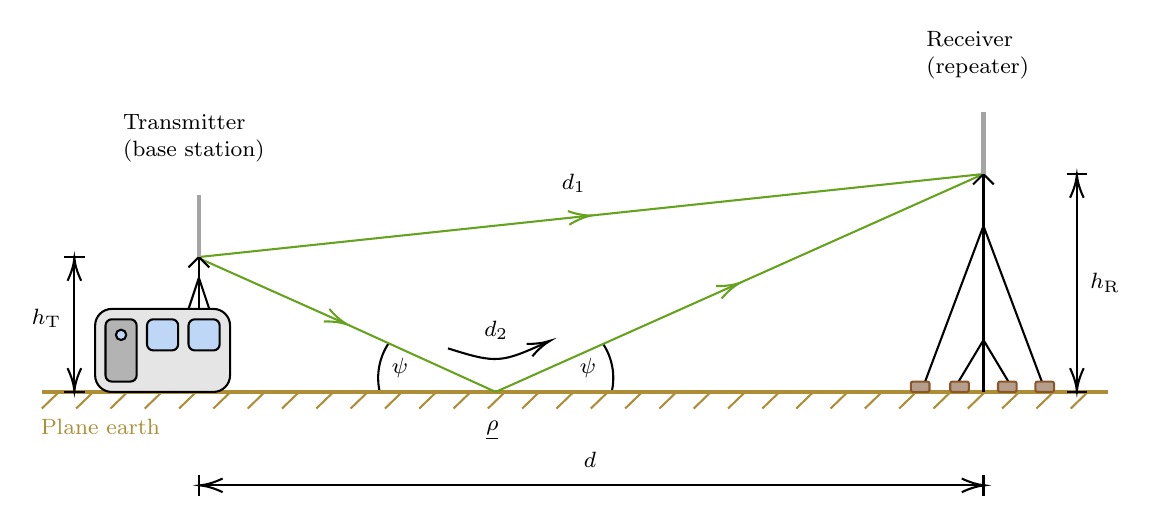
\begin{tikzpicture}[x=0.75pt,y=0.75pt,yscale=-1,xscale=1]
%uncomment if require: \path (0,876); %set diagram left start at 0, and has height of 876

%Shape: Arc [id:dp15338331881086464] 
\draw  [draw opacity=0] (340.87,690.02) .. controls (341.8,685.99) and (341.92,681.69) .. (341.05,677.36) .. controls (340.27,673.48) and (338.78,669.92) .. (336.73,666.79) -- (311.63,683.25) -- cycle ; \draw   (340.87,690.02) .. controls (341.8,685.99) and (341.92,681.69) .. (341.05,677.36) .. controls (340.27,673.48) and (338.78,669.92) .. (336.73,666.79) ;
%Shape: Arc [id:dp6996067112202611] 
\draw  [draw opacity=0] (229.13,689.98) .. controls (228.2,685.94) and (228.08,681.64) .. (228.95,677.32) .. controls (229.74,673.35) and (231.29,669.72) .. (233.4,666.55) -- (258.37,683.2) -- cycle ; \draw   (229.13,689.98) .. controls (228.2,685.94) and (228.08,681.64) .. (228.95,677.32) .. controls (229.74,673.35) and (231.29,669.72) .. (233.4,666.55) ;
%Straight Lines [id:da4849283455814688] 
\draw    (142,730) -- (142,740) ;
%Straight Lines [id:da7410756286600795] 
\draw    (520,730) -- (520,740) ;
%Straight Lines [id:da9884557143123041] 
\draw    (144.5,735) -- (518.5,735) ;
\draw [shift={(520.5,735)}, rotate = 180] [color={rgb, 255:red, 0; green, 0; blue, 0 }  ][line width=0.75]    (10.93,-3.29) .. controls (6.95,-1.4) and (3.31,-0.3) .. (0,0) .. controls (3.31,0.3) and (6.95,1.4) .. (10.93,3.29)   ;
\draw [shift={(142.5,735)}, rotate = 0] [color={rgb, 255:red, 0; green, 0; blue, 0 }  ][line width=0.75]    (10.93,-3.29) .. controls (6.95,-1.4) and (3.31,-0.3) .. (0,0) .. controls (3.31,0.3) and (6.95,1.4) .. (10.93,3.29)   ;
%Straight Lines [id:da6201954809627948] 
\draw [color={rgb, 255:red, 173; green, 142; blue, 55 }  ,draw opacity=1 ][fill={rgb, 255:red, 139; green, 87; blue, 42 }  ,fill opacity=1 ][line width=1.5]    (66.3,690) -- (430,690) ;
%Straight Lines [id:da06147530745502938] 
\draw [color={rgb, 255:red, 173; green, 142; blue, 55 }  ,draw opacity=1 ]   (74.59,690) -- (66.32,697.99) ;
%Straight Lines [id:da23007865791418336] 
\draw [color={rgb, 255:red, 173; green, 142; blue, 55 }  ,draw opacity=1 ]   (91.12,690) -- (82.85,697.99) ;
%Straight Lines [id:da767472737068108] 
\draw [color={rgb, 255:red, 173; green, 142; blue, 55 }  ,draw opacity=1 ]   (107.65,690) -- (99.38,697.99) ;
%Straight Lines [id:da13777850468332842] 
\draw [color={rgb, 255:red, 173; green, 142; blue, 55 }  ,draw opacity=1 ]   (124.18,690) -- (115.91,697.99) ;
%Straight Lines [id:da6751673575123742] 
\draw [color={rgb, 255:red, 173; green, 142; blue, 55 }  ,draw opacity=1 ]   (140.71,690) -- (132.44,697.99) ;
%Straight Lines [id:da9392755627171439] 
\draw [color={rgb, 255:red, 173; green, 142; blue, 55 }  ,draw opacity=1 ]   (157.24,690) -- (148.98,697.99) ;
%Straight Lines [id:da619671077470155] 
\draw [color={rgb, 255:red, 173; green, 142; blue, 55 }  ,draw opacity=1 ]   (173.77,690) -- (165.51,697.99) ;
%Straight Lines [id:da7290786911993896] 
\draw [color={rgb, 255:red, 173; green, 142; blue, 55 }  ,draw opacity=1 ]   (190.3,690) -- (182.04,697.99) ;
%Straight Lines [id:da4719174732926148] 
\draw [color={rgb, 255:red, 173; green, 142; blue, 55 }  ,draw opacity=1 ]   (206.83,690) -- (198.57,697.99) ;
%Straight Lines [id:da37628729746086] 
\draw [color={rgb, 255:red, 173; green, 142; blue, 55 }  ,draw opacity=1 ]   (223.36,690) -- (215.1,697.99) ;
%Straight Lines [id:da7920026566633553] 
\draw [color={rgb, 255:red, 173; green, 142; blue, 55 }  ,draw opacity=1 ]   (239.9,690) -- (231.63,697.99) ;
%Straight Lines [id:da6395101589775403] 
\draw [color={rgb, 255:red, 173; green, 142; blue, 55 }  ,draw opacity=1 ]   (256.43,690) -- (248.16,697.99) ;
%Straight Lines [id:da44232178865498684] 
\draw [color={rgb, 255:red, 173; green, 142; blue, 55 }  ,draw opacity=1 ]   (272.96,690) -- (264.69,697.99) ;
%Straight Lines [id:da35147828396454206] 
\draw [color={rgb, 255:red, 173; green, 142; blue, 55 }  ,draw opacity=1 ]   (289.49,690) -- (281.22,697.99) ;
%Straight Lines [id:da9217031911008662] 
\draw [color={rgb, 255:red, 173; green, 142; blue, 55 }  ,draw opacity=1 ]   (306.02,690) -- (297.75,697.99) ;
%Straight Lines [id:da2737629358231022] 
\draw [color={rgb, 255:red, 173; green, 142; blue, 55 }  ,draw opacity=1 ]   (322.55,690) -- (314.28,697.99) ;
%Straight Lines [id:da49095056220419875] 
\draw [color={rgb, 255:red, 173; green, 142; blue, 55 }  ,draw opacity=1 ]   (339.08,690) -- (330.81,697.99) ;
%Straight Lines [id:da9520266987449595] 
\draw [color={rgb, 255:red, 173; green, 142; blue, 55 }  ,draw opacity=1 ]   (355.61,690) -- (347.35,697.99) ;
%Straight Lines [id:da16568942576886259] 
\draw [color={rgb, 255:red, 173; green, 142; blue, 55 }  ,draw opacity=1 ]   (372.14,690) -- (363.88,697.99) ;
%Straight Lines [id:da4761808664553333] 
\draw [color={rgb, 255:red, 173; green, 142; blue, 55 }  ,draw opacity=1 ]   (388.67,690) -- (380.41,697.99) ;
%Straight Lines [id:da9228454528853451] 
\draw [color={rgb, 255:red, 173; green, 142; blue, 55 }  ,draw opacity=1 ]   (405.2,690) -- (396.94,697.99) ;
%Straight Lines [id:da5583266146555903] 
\draw [color={rgb, 255:red, 173; green, 142; blue, 55 }  ,draw opacity=1 ]   (421.73,690) -- (413.47,697.99) ;
%Straight Lines [id:da9492432558041424] 
\draw [color={rgb, 255:red, 173; green, 142; blue, 55 }  ,draw opacity=1 ][fill={rgb, 255:red, 139; green, 87; blue, 42 }  ,fill opacity=1 ][line width=1.5]    (430,690) -- (580,690) ;
%Straight Lines [id:da012970148931068515] 
\draw [color={rgb, 255:red, 173; green, 142; blue, 55 }  ,draw opacity=1 ]   (454.59,690) -- (446.32,697.99) ;
%Straight Lines [id:da8540196618758502] 
\draw [color={rgb, 255:red, 173; green, 142; blue, 55 }  ,draw opacity=1 ]   (471.12,690) -- (462.85,697.99) ;
%Straight Lines [id:da8712910446329858] 
\draw [color={rgb, 255:red, 173; green, 142; blue, 55 }  ,draw opacity=1 ]   (487.65,690) -- (479.38,697.99) ;
%Straight Lines [id:da47124045950262605] 
\draw [color={rgb, 255:red, 173; green, 142; blue, 55 }  ,draw opacity=1 ]   (504.18,690) -- (495.91,697.99) ;
%Straight Lines [id:da5090861497391432] 
\draw [color={rgb, 255:red, 173; green, 142; blue, 55 }  ,draw opacity=1 ]   (520.71,690) -- (512.44,697.99) ;
%Straight Lines [id:da23715254956587994] 
\draw [color={rgb, 255:red, 173; green, 142; blue, 55 }  ,draw opacity=1 ]   (537.24,690) -- (528.98,697.99) ;
%Straight Lines [id:da290192241167754] 
\draw [color={rgb, 255:red, 173; green, 142; blue, 55 }  ,draw opacity=1 ]   (553.77,690) -- (545.51,697.99) ;
%Straight Lines [id:da8622271615438304] 
\draw [color={rgb, 255:red, 173; green, 142; blue, 55 }  ,draw opacity=1 ]   (438.06,690) -- (429.79,697.99) ;
%Straight Lines [id:da035064651647806366] 
\draw [color={rgb, 255:red, 173; green, 142; blue, 55 }  ,draw opacity=1 ]   (570.3,690) -- (562.04,697.99) ;
%Straight Lines [id:da4011183020989364] 
\draw    (520,610) -- (490,690) ;
%Straight Lines [id:da27387454247993626] 
\draw    (520,610) -- (550,690) ;
%Straight Lines [id:da9736829818872206] 
\draw [color={rgb, 255:red, 0; green, 0; blue, 0 }  ,draw opacity=1 ]   (505,690) -- (520,665) ;
%Straight Lines [id:da7245451240532392] 
\draw [color={rgb, 255:red, 0; green, 0; blue, 0 }  ,draw opacity=1 ]   (535,690) -- (520,665) ;
%Straight Lines [id:da9897402100333932] 
\draw [color={rgb, 255:red, 0; green, 0; blue, 0 }  ,draw opacity=1 ]   (520,570) -- (520,690) ;
%Straight Lines [id:da13588456690109108] 
\draw    (77,625) -- (87,625) ;
%Straight Lines [id:da3556223533172955] 
\draw    (82,627.5) -- (82,687.5) ;
\draw [shift={(82,689.5)}, rotate = 270] [color={rgb, 255:red, 0; green, 0; blue, 0 }  ][line width=0.75]    (10.93,-3.29) .. controls (6.95,-1.4) and (3.31,-0.3) .. (0,0) .. controls (3.31,0.3) and (6.95,1.4) .. (10.93,3.29)   ;
\draw [shift={(82,625.5)}, rotate = 90] [color={rgb, 255:red, 0; green, 0; blue, 0 }  ][line width=0.75]    (10.93,-3.29) .. controls (6.95,-1.4) and (3.31,-0.3) .. (0,0) .. controls (3.31,0.3) and (6.95,1.4) .. (10.93,3.29)   ;
%Straight Lines [id:da2914330006317636] 
\draw    (570,585) -- (560,585) ;
%Straight Lines [id:da8173647824143173] 
\draw    (565,587.5) -- (565,687.5) ;
\draw [shift={(565,689.5)}, rotate = 270] [color={rgb, 255:red, 0; green, 0; blue, 0 }  ][line width=0.75]    (10.93,-3.29) .. controls (6.95,-1.4) and (3.31,-0.3) .. (0,0) .. controls (3.31,0.3) and (6.95,1.4) .. (10.93,3.29)   ;
\draw [shift={(565,585.5)}, rotate = 90] [color={rgb, 255:red, 0; green, 0; blue, 0 }  ][line width=0.75]    (10.93,-3.29) .. controls (6.95,-1.4) and (3.31,-0.3) .. (0,0) .. controls (3.31,0.3) and (6.95,1.4) .. (10.93,3.29)   ;
%Straight Lines [id:da1253612915505431] 
\draw    (570,690) -- (560,690) ;
%Straight Lines [id:da8984347678903521] 
\draw    (77,690) -- (87,690) ;
%Rounded Rect [id:dp03180466193560205] 
\draw  [color={rgb, 255:red, 139; green, 87; blue, 42 }  ,draw opacity=1 ][fill={rgb, 255:red, 181; green, 159; blue, 140 }  ,fill opacity=1 ] (485,686) .. controls (485,685.45) and (485.45,685) .. (486,685) -- (493,685) .. controls (493.55,685) and (494,685.45) .. (494,686) -- (494,689) .. controls (494,689.55) and (493.55,690) .. (493,690) -- (486,690) .. controls (485.45,690) and (485,689.55) .. (485,689) -- cycle ;
%Rounded Rect [id:dp451357267838828] 
\draw  [color={rgb, 255:red, 139; green, 87; blue, 42 }  ,draw opacity=1 ][fill={rgb, 255:red, 181; green, 159; blue, 140 }  ,fill opacity=1 ] (504,686) .. controls (504,685.45) and (504.45,685) .. (505,685) -- (512,685) .. controls (512.55,685) and (513,685.45) .. (513,686) -- (513,689) .. controls (513,689.55) and (512.55,690) .. (512,690) -- (505,690) .. controls (504.45,690) and (504,689.55) .. (504,689) -- cycle ;
%Rounded Rect [id:dp49767959341929235] 
\draw  [color={rgb, 255:red, 139; green, 87; blue, 42 }  ,draw opacity=1 ][fill={rgb, 255:red, 181; green, 159; blue, 140 }  ,fill opacity=1 ] (545,686) .. controls (545,685.45) and (545.45,685) .. (546,685) -- (553,685) .. controls (553.55,685) and (554,685.45) .. (554,686) -- (554,689) .. controls (554,689.55) and (553.55,690) .. (553,690) -- (546,690) .. controls (545.45,690) and (545,689.55) .. (545,689) -- cycle ;
%Rounded Rect [id:dp2760334360681225] 
\draw  [color={rgb, 255:red, 139; green, 87; blue, 42 }  ,draw opacity=1 ][fill={rgb, 255:red, 181; green, 159; blue, 140 }  ,fill opacity=1 ] (527,686) .. controls (527,685.45) and (527.45,685) .. (528,685) -- (535,685) .. controls (535.55,685) and (536,685.45) .. (536,686) -- (536,689) .. controls (536,689.55) and (535.55,690) .. (535,690) -- (528,690) .. controls (527.45,690) and (527,689.55) .. (527,689) -- cycle ;
%Straight Lines [id:da3373219558759375] 
\draw [color={rgb, 255:red, 101; green, 162; blue, 30 }  ,draw opacity=1 ]   (402.5,637.5) -- (520,585) ;
%Curve Lines [id:da5027137859040653] 
\draw    (262,669) .. controls (285.59,676.47) and (287.58,676.03) .. (309.51,666.1) ;
\draw [shift={(311.24,665.32)}, rotate = 515.62] [color={rgb, 255:red, 0; green, 0; blue, 0 }  ][line width=0.75]    (10.93,-3.29) .. controls (6.95,-1.4) and (3.31,-0.3) .. (0,0) .. controls (3.31,0.3) and (6.95,1.4) .. (10.93,3.29)   ;
%Straight Lines [id:da2871504343231346] 
\draw [color={rgb, 255:red, 101; green, 162; blue, 30 }  ,draw opacity=1 ]   (143.14,626.07) -- (211.67,656.68) ;
\draw [shift={(213.5,657.5)}, rotate = 204.07] [color={rgb, 255:red, 101; green, 162; blue, 30 }  ,draw opacity=1 ][line width=0.75]    (10.93,-3.29) .. controls (6.95,-1.4) and (3.31,-0.3) .. (0,0) .. controls (3.31,0.3) and (6.95,1.4) .. (10.93,3.29)   ;
%Straight Lines [id:da10153281804164327] 
\draw [color={rgb, 255:red, 101; green, 162; blue, 30 }  ,draw opacity=1 ]   (142,625) -- (329.01,605.21) ;
\draw [shift={(331,605)}, rotate = 533.96] [color={rgb, 255:red, 101; green, 162; blue, 30 }  ,draw opacity=1 ][line width=0.75]    (10.93,-3.29) .. controls (6.95,-1.4) and (3.31,-0.3) .. (0,0) .. controls (3.31,0.3) and (6.95,1.4) .. (10.93,3.29)   ;
%Straight Lines [id:da9243245263761997] 
\draw [color={rgb, 255:red, 101; green, 162; blue, 30 }  ,draw opacity=1 ]   (331,605) -- (520,585) ;
%Straight Lines [id:da37753849790320726] 
\draw [color={rgb, 255:red, 101; green, 162; blue, 30 }  ,draw opacity=1 ]   (285,690) -- (400.67,638.32) ;
\draw [shift={(402.5,637.5)}, rotate = 515.9200000000001] [color={rgb, 255:red, 101; green, 162; blue, 30 }  ,draw opacity=1 ][line width=0.75]    (10.93,-3.29) .. controls (6.95,-1.4) and (3.31,-0.3) .. (0,0) .. controls (3.31,0.3) and (6.95,1.4) .. (10.93,3.29)   ;
%Straight Lines [id:da5377616802262684] 
\draw [color={rgb, 255:red, 101; green, 162; blue, 30 }  ,draw opacity=1 ]   (213.5,657.5) -- (285,690) ;
%Straight Lines [id:da7429729161371501] 
\draw    (515,590) -- (520,585) ;
%Straight Lines [id:da10327988326649606] 
\draw    (520,585) -- (525,590) ;
%Straight Lines [id:da29587755982689723] 
\draw [color={rgb, 255:red, 164; green, 164; blue, 164 }  ,draw opacity=1 ][line width=1.5]    (520,555) -- (520,585) ;
%Straight Lines [id:da9451254669725766] 
\draw [color={rgb, 255:red, 0; green, 0; blue, 0 }  ,draw opacity=1 ]   (137,650) -- (142,635) ;
%Straight Lines [id:da7504831693397569] 
\draw [color={rgb, 255:red, 0; green, 0; blue, 0 }  ,draw opacity=1 ]   (147,650) -- (142,635) ;
%Straight Lines [id:da4778455848429135] 
\draw [color={rgb, 255:red, 0; green, 0; blue, 0 }  ,draw opacity=1 ]   (142,620) -- (142,650) ;
%Rounded Rect [id:dp912082830075883] 
\draw  [fill={rgb, 255:red, 229; green, 229; blue, 229 }  ,fill opacity=1 ] (92,658) .. controls (92,653.58) and (95.58,650) .. (100,650) -- (149,650) .. controls (153.42,650) and (157,653.58) .. (157,658) -- (157,682) .. controls (157,686.42) and (153.42,690) .. (149,690) -- (100,690) .. controls (95.58,690) and (92,686.42) .. (92,682) -- cycle ;
%Rounded Rect [id:dp5521679148983523] 
\draw  [fill={rgb, 255:red, 179; green, 179; blue, 179 }  ,fill opacity=1 ] (97,658) .. controls (97,656.34) and (98.34,655) .. (100,655) -- (109,655) .. controls (110.66,655) and (112,656.34) .. (112,658) -- (112,682) .. controls (112,683.66) and (110.66,685) .. (109,685) -- (100,685) .. controls (98.34,685) and (97,683.66) .. (97,682) -- cycle ;
%Shape: Circle [id:dp12394399539515244] 
\draw  [fill={rgb, 255:red, 190; green, 215; blue, 246 }  ,fill opacity=1 ] (102,662.5) .. controls (102,661.12) and (103.12,660) .. (104.5,660) .. controls (105.88,660) and (107,661.12) .. (107,662.5) .. controls (107,663.88) and (105.88,665) .. (104.5,665) .. controls (103.12,665) and (102,663.88) .. (102,662.5) -- cycle ;

%Rounded Rect [id:dp6421651030261453] 
\draw  [fill={rgb, 255:red, 190; green, 215; blue, 246 }  ,fill opacity=1 ] (117,658) .. controls (117,656.34) and (118.34,655) .. (120,655) -- (129,655) .. controls (130.66,655) and (132,656.34) .. (132,658) -- (132,667) .. controls (132,668.66) and (130.66,670) .. (129,670) -- (120,670) .. controls (118.34,670) and (117,668.66) .. (117,667) -- cycle ;
%Rounded Rect [id:dp31354760153476446] 
\draw  [fill={rgb, 255:red, 190; green, 215; blue, 246 }  ,fill opacity=1 ] (137,658) .. controls (137,656.34) and (138.34,655) .. (140,655) -- (149,655) .. controls (150.66,655) and (152,656.34) .. (152,658) -- (152,667) .. controls (152,668.66) and (150.66,670) .. (149,670) -- (140,670) .. controls (138.34,670) and (137,668.66) .. (137,667) -- cycle ;
%Straight Lines [id:da0782772154376139] 
\draw    (142,625) -- (147,630) ;
%Straight Lines [id:da8311058955990167] 
\draw    (142,625) -- (137,630) ;
%Straight Lines [id:da8470826261048678] 
\draw [color={rgb, 255:red, 164; green, 164; blue, 164 }  ,draw opacity=1 ][line width=1.5]    (142,595) -- (142,625) ;

% Text Node
\draw (326,717.4) node [anchor=north west][inner sep=0.75pt]  [font=\footnotesize]  {$d$};
% Text Node
\draw (64.3,701.57) node [anchor=north west][inner sep=0.75pt]  [font=\footnotesize,color={rgb, 255:red, 173; green, 142; blue, 55 }  ,opacity=1 ] [align=left] {Plane earth};
% Text Node
\draw (60,648.4) node [anchor=north west][inner sep=0.75pt]  [font=\footnotesize]  {$h_{\mathrm{T}}$};
% Text Node
\draw (570,631.4) node [anchor=north west][inner sep=0.75pt]  [font=\footnotesize]  {$h_{\mathrm{R}}$};
% Text Node
\draw (315.4,583.4) node [anchor=north west][inner sep=0.75pt]  [font=\footnotesize]  {$d_{1}$};
% Text Node
\draw (278,654.4) node [anchor=north west][inner sep=0.75pt]  [font=\footnotesize]  {$d_{2}$};
% Text Node
\draw (279,702.4) node [anchor=north west][inner sep=0.75pt]  [font=\footnotesize]  {$\underline{\rho }$};
% Text Node
\draw (324,672.4) node [anchor=north west][inner sep=0.75pt]  [font=\footnotesize]  {$\psi $};
% Text Node
\draw (233.44,672.4) node [anchor=north west][inner sep=0.75pt]  [font=\footnotesize]  {$\psi $};
% Text Node
\draw (491,515) node [anchor=north west][inner sep=0.75pt]  [font=\footnotesize] [align=left] {Receiver\\(repeater)};
% Text Node
\draw (104,555) node [anchor=north west][inner sep=0.75pt]  [font=\footnotesize] [align=left] {Transmitter\\(base station)};


\end{tikzpicture}

	\caption{Illustration of the plane earth signal budget. (Recreated from: \cite{Parsons:2000, Glover:2010, Goiser:2019})}
	\label{fig:tikz_plane_earth_signal_budget}
\end{figure}
The latter can be obtained from the equation (\ref{eq:reflection_coeff}), where $\varepsilon_\mathrm{r}$ in $\left(1\right)$ is the \emph{relative dielectric constant} of the Earth, $\varepsilon_\mathrm{0}$ in $\left(\mathrm{AsV^{-1}m^{-1}}\right)$ is the \emph{dielectric constant of free space}, $\sigma$ in $\left(\mathrm{\Omega^{-1}}\right)$ is the \emph{conductivity} of the Earth and $\omega = 2\pi \, f_\sim$ is the \emph{angular frequency} in $\left(\mathrm{s^{-1}}\right)$.
\begin{equation} \label{eq:reflection_coeff}
	\centering
	\underline{\rho} = \dfrac{\left(\varepsilon_\mathrm{r} - jx \right) \sin \psi - \sqrt{\left(\varepsilon_\mathrm{r} - jx \right) - \cos^2 \psi}}{\left(\varepsilon_\mathrm{r} - jx \right) \sin \psi + \sqrt{\left(\varepsilon_\mathrm{r} - jx \right) - \cos^2 \psi}}\text{,} \quad \text{with } x = \dfrac{\sigma}{\omega \, \varepsilon_0}
\end{equation}
Based on $\underline{\rho}$, the field strength at the receiving antenna changes with the complex factor:
\begin{equation} \label{eq:field_strength}
	\centering
	\underline{F} = 1 + \underline{\rho} \exp \left( - j \Theta \right)\text{.}
\end{equation}
The \emph{phase difference} $\Theta$ in $\left(\mathrm{rad}\right)$ -- which occurs due to the reflection of the electromagnetic wave -- can be derived from the figure \ref{fig:tikz_plane_earth_signal_budget} as shown below:
\begin{equation} \label{eq:phase_difference}
	\centering
	\Theta = \dfrac{4\pi \, h_\mathrm{T} \, h_\mathrm{R}}{\lambda_\sim \, d}\text{.}
\end{equation}
If the angle of incidence $\psi$ is small, which is the case for $d \gg h_\mathrm{T}, h_\mathrm{R}$, a perfect reflection of the electromagnetic wave can be assumed, hence $\underline{\rho} = \exp(j\pi) = -1$.\footnote{It can be seen that the phase difference $\Theta$ is small for $d \gg h_\mathrm{T}, h_\mathrm{R}$.} This is because the E-field for the \emph{transversal magnetic} (TM) mode is perpendicular to the plane when $\psi$ is small \cite{Mecklenbrauker:2017}. As a result, the squared absolute value of the complex factor, which now represents the power increase at the receiving antenna compared to free space propagation, can be simplified to:
\begin{equation} \label{eq:field_strength}
	\centering
	\left|\underline{F}\right|^2 = 4 \left| \sin^2 \left(\dfrac{\Theta}{2}\right) \right| = 4 \sin^2 \left(\dfrac{2\pi \, h_\mathrm{T} \, h_\mathrm{R}}{\lambda_\sim \, d}\right) \text{,} \quad \text{for } \underline{\rho} = -1\text{.}
\end{equation}
By multiplying the result from the equation (\ref{eq:field_strength}) with the right side of the equation (\ref{eq:free_space}), the available power at the receiving antenna for plane earth propagation results in: 
\begin{equation} \label{eq:plane_earth}
	\centering
	\begin{aligned}
	P_\mathrm{R} & = P_\mathrm{T} \left(\dfrac{\lambda_\sim}{4 \pi \, d}\right)^2 L_\mathrm{R} \, L_\mathrm{T} \, G_\mathrm{R} \, G_\mathrm{T} \, \left|\underline{F}\right|^2 \\
				 & = 4P_\mathrm{T} \left(\dfrac{\lambda_\sim}{4 \pi \, d}\right)^2 L_\mathrm{R} \, L_\mathrm{T} \, G_\mathrm{R} \, G_\mathrm{T} \sin^2 \left(\dfrac{2\pi \, h_\mathrm{T} \, h_\mathrm{R}}{\lambda_\sim \, d}\right)\text{.}
	\end{aligned}
\end{equation}
Finally, since $d \gg h_\mathrm{T} \text{, } h_\mathrm{R}$ applies, the sine in the equation (\ref{eq:plane_earth}) can be approximated with $\sin x \approx x$, from which the \emph{plane earth propagation equation} is derived:
\begin{equation} \label{eq:plane_earth_approx}
	\centering
	P_\mathrm{R} = P_\mathrm{T} \left(\dfrac{h_\mathrm{T} \, h_\mathrm{R}}{d^2}\right)^2 L_\mathrm{R} \, L_\mathrm{T} \, G_\mathrm{R} \, G_\mathrm{T}\text{, } \quad \text{for } d \gg h_\mathrm{T}\text{, } h_\mathrm{R}\text{.}
\end{equation}
Expressed in decibels this equation can be written as:
\begin{equation} \label{eq:plane_earth_approx_db}
	\centering
	\begin{gathered}
	P_\mathrm{R,dBW} = P_\mathrm{T,dBW} + \overbrace{20\mathrm{dB} \cdot \log_{10} \left(\dfrac{h_\mathrm{T} \, h_\mathrm{R}}{d^2}\right)}^{\mathrm{-PEPL_{dB}}} - L_\mathrm{R,dB} - L_\mathrm{T,dB} + G_\mathrm{R,dBi} + G_\mathrm{T,dBi}\text{, } \\ \quad \text{for } d \gg h_\mathrm{T}\text{, } h_\mathrm{R}\text{.}
	\end{gathered}
\end{equation}
$\mathrm{PEPL_{dB}}$ is the \emph{plane earth path loss} in $\left(\mathrm{dB}\right)$ \cite{Parsons:2000, Glover:2010, Goiser:2019}.
\subsection{Martian application}
In the previous subsections, some important factors were neglected in order to provide a rough performance estimation of the voice communication system on Earth. For an application on Mars these factors should be considered when designing such a system. 

First, the influence of the internal noise of the components -- which is due to their thermal noise -- as well as the influence of the electromagnetic noise collected by the receiving antenna, must be considered. Antennas in the $30\mathrm{MHz}$ to $1\mathrm{GHz}$ range primarily pick up galactic noise which is caused by the radiation produced by electrons moving through the galactic magnetic field of the Milky Way. Due to the shape of the Milky Way and the location of the Earth within it, this type of noise is anisotropic in nature. It increases when the antenna is pointed directly at the center of the Milky Way. For a more detailed examination of the link budget of a voice communication system on Mars, the galactic noise affecting the system would have to be examined more closely. Because of the low temperatures on Mars, the thermal noise of the components and radio devices will probably be lower. However, due to the thinner atmosphere, the heat generated by these cannot be dissipated, which in turn increases the temperature of the system and thus its thermal noise. This problem must be solved with suitable cooling. For completeness it must be mentioned that interference caused by other missions or electrical devices on the surface of Mars or in its orbit should not be neglected when planning a voice communication system. Such interferences can be identified as man-made-noise \cite{Glover:2010, Goiser:2019, Kemmetmuller:2021}. 

Second, a topological map of the mission location can be created, on the basis of which a multipath propagation simulation is carried out so that the radio infrastructure can be optimally placed. In contrast to the voice communication system of the OeWF, which is constantly being set up at new mission locations, it is assumed that the radio infrastructure on Mars will only be set up once and then expanded with further missions. Thus, such an elaborate simulation of the multipath propoagation can be usefull. It is desirable to set up a functioning voice communication network with as little infrastructure as possible in order to save weight and minimize assembly time \cite{Ho:2002}.

Third, the propagation of VHF waves in relation to the Martian atmosphere must be investigated. The authors of \cite{Ho:2002} have found out that Mars has almost no intrinsic magnetic field, which means that the use of the ionosphere for wave propagation is very dependent on the time of day and the season. During the day, the ionosphere can be used as a reflector for global communication, whereas this may not be possible at night. The authors also assumed that the attenuation of a VHF signal due to the ionosphere is approximately $0,5\mathrm{dB}$. The effects of storms in the ionosphere have not yet been researched enough to make any statements about them.

Since the troposphere of Mars is very thin, it is believed that it has little effect on the propagation of electromagnetic waves \cite{Ho:2002}.

With regard to dust storms, the authors of \cite{Ho:2002} further state that due to the large wavelength of VHF signals, compared to the size of Martian dust particles -- with adiameter of $0,1\mathrm{mm}$ -- the signal attenuation is rather small. However, this still needs to be researched, as dust density also plays a major role. 

Fourth, the system must have sufficient redundancy so that a total failure is very unlikely. Loss of communication can potentially be dangerous for a crew during an ongoing mission. 





